\documentclass[a4paper,12pt,english,openright]{book}
\usepackage[doublespacing]{setspace}
%mettere oneside dopo la lingua per stampare solo fronte
\usepackage[T1]{fontenc}
\usepackage[utf8]{inputenc}
\usepackage{lscape}
\usepackage{graphicx}
\usepackage{epstopdf}
\usepackage[english]{babel}
\usepackage{lmodern}
\usepackage[T1]{fontenc}
\usepackage{floatrow}
\usepackage{titlesec}
\usepackage{tikz}
\usepackage{amsfonts,amsmath,amsthm,amssymb,stmaryrd,bbm,bm,commath,mathrsfs}
\usepackage{afterpage,wrapfig}
\usepackage{booktabs,array,multirow} 
\usepackage{subfigure,longtable}
\usepackage{capt-of}
\usepackage{appendix}
\usepackage{chngcntr}
\usepackage{etoolbox}
\usepackage{lipsum}
\usepackage[square,numbers]{natbib}
\usepackage[sectionbib]{chapterbib}

% \usepackage[square,numbers]{natbib}
\bibliographystyle{plainnat}

\newcounter{appendix}[chapter]
\usepackage{chngcntr}
\usepackage{marginnote,datetime,enumitem,rotating,fancyvrb}
\usepackage[inner=2.5cm,outer=2.5cm,bottom=4cm,top=3cm]{geometry}
%\linespread{1.3} %interlinea 
\usepackage{caption}
\usepackage{tikz}
\tikzset{
	position label/.style={
		below = 3pt,
		text height = 1.5ex,
		text depth = 1ex
	},
	brace/.style={
		decoration={brace, mirror},
		decorate
	}
}
\usetikzlibrary{arrows,positioning,patterns,decorations.pathreplacing} 
\usepackage{capt-of}
\usepackage{url}
\usepackage{hyperref}

\newtheorem{definition}{Definition}
\newtheorem{theorem}{Theorem}
\newtheorem{proposition}{Proposition}
\newtheorem{corollary}{Corollary}
\newtheorem{lem}{Lemma}
% \newtheorem{proof}{Proof}
\newtheorem{example}{Example}
\newtheorem{remark}{Remark}
\author{}
%\input{Preamble}
\newcommand{\EE}{\mathbb{E}}
\newtheorem{defi}{Definition}[section]
\newtheorem{prop}{Proposition}[section]
\newcommand{\dd}{\mathrm{d}}

\newenvironment{abstract}{%
\clearpage\thispagestyle{empty}\vspace*{3\baselineskip}
\begin{center}\textbf\abstractname\end{center}
\begin{quotation}
}{\end{quotation}\clearpage}

\begin{document}
\title{Swedish Multigeneration Registries}
\author{Maria Veronica Vinattieri}
\maketitle
\section*{Cleaning Registries}
I first report what is contained by the available registries, and how they have been modified to be merged together: 
\begin{itemize}
    \item DEMOGRAPHY REGISTRY: 
there are information about the birthday (\texttt{FODELSEMAN}) and the death date (\texttt{DodDatum}) of the subject. There are no ties, so every subject appears with his id number (\texttt{LOPNR}) once: each row is a different subject. The majority of next registries will be modified to have not ties on the id number of subjects (so that each subject coincides with a unique row), so that later the datasets can be merged together and have for each row one subject with complete information on both personal and relatives' survival details. 
\item BIOMOR REGISTRY: it contains information about the biological mother of the subject. No ties have been found here, as we could expect, indeed each subject must have a unique biological mother and appears once in the dataset.
\item SYSKON REGISTRY: it contains the siblings relationship one to one. There are ties: each subject is repeated for how many siblings it has. Plus, the information on the relationship is given (full sisters, half sister from the mother side (with same father or missing information on the father), half sister from the father side (with same mother or missing information on the mother). First of all we select only the females, because we are interested in the sisters. And we select the full sisters for several reason: the environmental factor is not as strong as the genetic factor (the same childhood place is not a cause of familiar aggregation of breast cancer) \cite{czene2002environmental}, and second, we want to have also indirectly the genetic information from the father that the sisters can share only if they have the same father. Now the dataset contains only full sisters. To remove the ties and have a unique row for each subject we move from a multiple rows structure to a multiple column structure. We build columns as many as the maximum number of sisters in a family, that is twelve (thirteen daughters indeed). The columns have name "Sister 1" ... "Sister 12" and their value correspond to the sister's id number if there is that one (first, second, ..., twelfth) taken from the rows, otherwise there is a missing value. Who is in the dataset and passed the filtering step has a least one sister, so the column of the first sister should be completely full information. From the second on, the number of missing value is clearly increasing. 
\item CANCER REGISTRY: it has all the different cancer types recorded in it, so we want to first select for breast cancer. The international classification of disease (ICD) is used to identify the breast cancer. Especially, the ICD7 identifies breast cancer through every code that starts with ``170'' \cite{icd7}, ICD9 with ``174'' \cite{icd9}, both ICDO10 and ICDO3 with ``C050'' \cite{icdo10, icdo3}. We find complete information on ICD7, so we decide to filter for that variable. Once filtered, we check whether the classification on the other variables coincide. We find five special cases in the other coding scales: one woman is identified as having a malignant neoplasm in genital organs (ICD9 = 1844), two with a non-specified neoplasm (ICD = 1991, ICD10 = C809), one with a placenta neoplasm (ICD3 = C589), and one with lymph nodes of axilla or arm neoplasm (ICD3 = C773). \textcolor{red}{reference} Due to the nature of breast cancer, as part of genitalia, and given that tumor mass in the lymph nodes start from a breast cancer, we keep four of these special cases. On the contrary, we remove the case of placenta neoplasm in ICDO3 because it does not coincide with a breast cancer case in ICD7. 

Moreover, this dataset has multiple rows for each subject, so we find the id number potentially in multiple rows. This is due to the breast cancer development through different visits. Since we are interested in the first invasive cancer occurrence the time to breast cancer coincides with the visit time when the breast cancer has been detected for the first time. The computational process of the time-to-breast cancer selection follows the steps: first, I selected the first breast cancer diagnosis time; after that, I noticed there were ties, meaning that there were multiple rows with the same id number and the same day of visit. This means that a patient could have undertaken two or more visits the same day in the hospital and then multiple visits have been recorded. For these cases, I selected the first visit in the dataset appearance, without loss of any information. Indeed, we only need the date of the breast cancer onset that is equivalent among the visits in the same day, clearly. What we lose are the cancer details that might change from visit to visit, even in the same day of analysis. But, this is out of our interest so far. Aside from the information on the day, we are interested in the invasive nature of the cancer (\texttt{BEN}). Indeed, we consider ductal carcinoma in-situ (DCIS, \texttt{BEN=3}) cancers as censoring events, and only invasive breast cancer as our event of interest. Also, when there are cases with a DCIS onset and later an invasive breast cancer they are censored at the DCIS time. Indeed, when a DCIS is found it is treated in some way so the natural breast cancer development is modified and biased by the DCIS treatment. Consequently, we cannot take into analysis a time-to-breast cancer appeared after a recorded DCIS time back. After removing the ties, there are 20216 cases of DCIS on a total of 265756, the 7$\%$, as in the univariate dataset. While, in the univariate reduced birthday window dataset there will be the 14$\%$. Beside this information we do not select the other breast cancer details, basically on TMN, because they are out of our interest. But, they are available in the source dataset anytime. 

\item MIGRATION REGISTRY: 
subjects can emigrate (\texttt{Unt}) or immigrate (\texttt{Int}) multiple times in and out from and to Sweden. Each move is recorded in a row with the information on emigration/immigration. This means that the id number of subjects might be repeated as many times as she moves in and out. To remove the ties we move from a multiple rows structure to a multiple columns structure. Multiple columns have been built as many as the maximum number of movements by a subject in the dataset. Then, each row information has been moved to the corrispoding column, identified with the movement time and the nature of it between emigration/immigration. So, every subject has now one row and multiple columns with the date of her movements (if happened, otherwise missing value). For example, \texttt{Unt1} means the first emigration, while \texttt{Int2} means the first immigration, back to Sweden after a recorded emigration, where the ``2'' indicates that is the second movement of the subject. 
\end{itemize}

\section*{Building Survival Variables}
\begin{itemize}
\item OBSERVED DATE: it is the first event among diagnosis time, emigration time, death, or end of the study. The last invasive breast cancer visit has been taken as the end of follow-up for all, that is on the 30 December 2016. We have information until the 31st December 2018 but there will be censored observations with probability 1 without bringing additional information to the problem, so the follow-up ends for all two years before. There are some cases of both information on diagnosis and emigration, or diagnosis and death. But usually there are not both info about emigration and death because one totally excludes the observation and recording of the other. Several	subjects have not information on any of these three, so the date of the end of the study is their observed date. We set the format of this variable to ``YYYY-MM-DD''. Most of the observations have this format, but there are some cases that we modify by hand not to lose information and to work with them properly at the same time. There are nine special cases: three cases were on the 29th of February but R causes an error with them. Now they have been modified to 28th of February; one case had ``0'' as date, and it has been modified with the end of follow-up; four dates were in the format ``YYYY-00-00'' so they have been added of the middle day, 15th, of the middle month over the year, June. The operation has been consisted in adding +615 to the format ``YYYY0000'' and then transforming it in ``YYYY-MM-DD''; similarly, for the only case without the day in the format ``YYYY-MM-00'', it has been adjusted the day to coincide with the 15the of that month. An other possible choice might be randomly sampling a day of the month between the 1 and the 28 (or 30, or 31) in according to which month. 
\item OBSERVED TIME: it is the follow-up length, i.e. the time gap between the entering in the risk group and the exit day. Since the follow-up starts at birth and it ends the day of the observed date, as explained in the bullet point above, the observed time is the difference in days between birth and the first event that occurs. The observed time is easily modifiable in months of years difference. 
\item DELTA: it is the indicator of having observed the invasive breast cancer onset. I previously created a vector in the cancer registry that takes value one but for the cases where the cancer has been recorded as a DCIS. In that case delta takes value zero. At the merging step between the Cancer Registry and the Demographic Registry, the variable delta will contain missing values corresponding the the subject not included in the Cancer Registry. All the missing values are replaced with a zero because clearly those subjects hadn't experienced the breast cancer yet.
\item FH: it is the family history indicator of breast cancer among the available first-degree female relatives. The breast cancer of the other relatives must occur before the observed time of the main subject. We define as main subjects the women included in the dataset as observations (on the rows), and not only as relatives of a main subject (on the columns). If all the family members are missing, then the family history is missing, in all the other cases, with at least one relative in the family, the family history assumes value zero or one. When there are only censoring cases in the family before the observed time of the subject then the family history is negative, otherwise the family history is positive. If there were ties on the observed times between relatives, we do not consider a positive family history but a negative one. This means that the case of breast cancer must happen at least one day before the time of the analysis of the main subject to count as family history of breast cancer. Otherwise, there is no history. 

Lastly, we notice a consistent missing information on the mother issue. This is due to several reasons: there could be the adoptive mother recorded instead of the biological one or the main subject has born in the first years of the study and her mother is not recorded. However, a unexplained portion of missing mothers remains. 
\end{itemize}
\section*{Building the dataset}
First of all, I want to build a dataset where there are available the necessary information of all the women on: birthday, death, emigration, observed date, observed time and delta. 

All the registries that will be mentioned below has been cleaned as described in the previous section.

We start from the census where we get information on the birthday and the death time of all the individuals. We select only women (6633147). Then, we merge this dataset with the breast cancer registry, where most importantly we get the information of the time of breast cancer onset from. The result is a dataset with information on birthday, time of death (if occurred, otherwise missing value), time of breast cancer onset (if occurred, otherwise missing value), tumor nature between ductual carcinoma in-situ (DCIS) and invasive cancer, and a binary indicator of invasive breast cancer occurrence. Then, the information on the last emigration time has been added (if occurred, otherwise missing value) from the emigration registry. 

All the necessary information are now available to build the survival couple (observed time, indicator of having observed the event). We already have the latter, while the former is computed as the minimum time between the time of invasive breast cancer, death, last emigration or end of the follow-up for all that coincides with the 30 December 2016. Indeed, the newborn after the year 2016 have been removed in this step and the subjects available were reduced to 6515271. Since we are going to use this dataset several times later, I give to this dataset a name so that I can mention it: the ``Demographic Dataset (DD)''. This dataset has complete personal information on the subject, without knowing the family structure and the relatives' survival details. We build this part in the next paragraph. 

From the Mother Dataset we get information on the id number of the mother. Similarly, from the Sister Dataset we get information on the id number of all of them for each subject. The columns of the mother and sisters' id were added to the dataset respecting the relationships row-wise. Up to this point the dataset has complete demographic information on the main subject from DD and, additionally, the id of mother and all sisters of the subject herself (if there are, otherwise missing value). Next, for all the subject's relatives we get the survival couple variables from DD. For each relative there are two additional columns in the dataset: the indicator of having observed the invasive breast cancer onset and the observed time. The final dataset has unique subjects' id on the row, and associated to her there are survival information of herself (from DD), the relatives' id and the corresponding survival information of them (from DD). We call this dataset the ``Multivariate Dataset (MD)'' to refer to the repeated information from relatives in the family. Indeed a mother of a sister could appear as a relative of a subject (in a column refer to the subject's row), and they may also appear as main subjects, with their survival information and their mother and sisters with survival information too. This information is redundant, so we want to keep only one subject per family. First of all for each mother, only one daughter is selected at random. Afterwards, for each family, now composed by a mother and on daughter, one of the two is selected at random. Due to this selection process it is guaranteed that the mother is selected with the probability $0.5$. Without this selection process, randomly sampling one subject per family would not give to the mother the probability up to $0.5$ if in the family there were two or more sisters. We did not want to lose a lot of mothers as main subjects. The dataset dimension reduced to 4,182,432. We call this dataset the ``Univariate Dataset (UD)''. Hence, we want to select a unique generation of women and, at the same time, a long time of follow-up to validate our methods later. Only women born between 1947 and 1976 are kept in the dataset, and the dimension is reduced to 1,068,181, that is still a consistent sample size to work with. The consort diagram of the dataset building is the following. 
\begin{figure}[ht]
\tikzset{every picture/.style={line width=0.75pt}} %set default line width to 0.75pt        
\begin{tikzpicture}[x=0.75pt,y=0.75pt,yscale=-1,xscale=1]
%uncomment if require: \path (0,235); %set diagram left start at 0, and has height of 235

%Straight Lines [id:da3965663235450416] 
\draw    (231,56) -- (231.59,83.75) ;
\draw [shift={(231.63,85.75)}, rotate = 268.78] [color={rgb, 255:red, 0; green, 0; blue, 0 }  ][line width=0.75]    (10.93,-3.29) .. controls (6.95,-1.4) and (3.31,-0.3) .. (0,0) .. controls (3.31,0.3) and (6.95,1.4) .. (10.93,3.29)   ;
%Straight Lines [id:da5350412613088747] 
\draw    (231.32,70.88) -- (436.63,71.74) ;
\draw [shift={(438.63,71.75)}, rotate = 180.24] [color={rgb, 255:red, 0; green, 0; blue, 0 }  ][line width=0.75]    (10.93,-3.29) .. controls (6.95,-1.4) and (3.31,-0.3) .. (0,0) .. controls (3.31,0.3) and (6.95,1.4) .. (10.93,3.29)   ;
%Straight Lines [id:da6781013778317039] 
\draw    (231,115) -- (231.59,142.75) ;
\draw [shift={(231.63,144.75)}, rotate = 268.78] [color={rgb, 255:red, 0; green, 0; blue, 0 }  ][line width=0.75]    (10.93,-3.29) .. controls (6.95,-1.4) and (3.31,-0.3) .. (0,0) .. controls (3.31,0.3) and (6.95,1.4) .. (10.93,3.29)   ;
%Straight Lines [id:da5677135778357121] 
\draw    (231.32,129.88) -- (441.63,129.75) ;
\draw [shift={(443.63,129.75)}, rotate = 179.97] [color={rgb, 255:red, 0; green, 0; blue, 0 }  ][line width=0.75]    (10.93,-3.29) .. controls (6.95,-1.4) and (3.31,-0.3) .. (0,0) .. controls (3.31,0.3) and (6.95,1.4) .. (10.93,3.29)   ;
%Straight Lines [id:da95691968340309] 
\draw    (230,174) -- (230.59,201.75) ;
\draw [shift={(230.63,203.75)}, rotate = 268.78] [color={rgb, 255:red, 0; green, 0; blue, 0 }  ][line width=0.75]    (10.93,-3.29) .. controls (6.95,-1.4) and (3.31,-0.3) .. (0,0) .. controls (3.31,0.3) and (6.95,1.4) .. (10.93,3.29)   ;
%Straight Lines [id:da021016050928771235] 
\draw    (230.32,188.88) -- (442.63,188.75) ;
\draw [shift={(444.63,188.75)}, rotate = 179.97] [color={rgb, 255:red, 0; green, 0; blue, 0 }  ][line width=0.75]    (10.93,-3.29) .. controls (6.95,-1.4) and (3.31,-0.3) .. (0,0) .. controls (3.31,0.3) and (6.95,1.4) .. (10.93,3.29)   ;

% Text Node
\draw (134,34) node [anchor=north west][inner sep=0.75pt]   [align=left] {initial sample (n = 6,633,147)};
% Text Node
\draw (451,54) node [anchor=north west][inner sep=0.75pt]   [align=left] {Excluded (n = 117,876) \\birthday after 31/12/2016};
% Text Node
\draw (41,93) node [anchor=north west][inner sep=0.75pt]   [align=left] {only women with birth within end of study (n = 6,515,271)};
% Text Node
\draw (451,110) node [anchor=north west][inner sep=0.75pt]   [align=left] {Excluded (n = 2,332,839)\\Only one subject per family};
% Text Node
\draw (118,151) node [anchor=north west][inner sep=0.75pt]   [align=left] {single family subject sample (n = 4,182,432)};
% Text Node
\draw (451,168) node [anchor=north west][inner sep=0.75pt]   [align=left] {Excluded (n = 3,114,251)\\birthday within 1947 and 1976};
% Text Node
\draw (170,213) node [anchor=north west][inner sep=0.75pt]   [align=left] {final sample (n = 1,068,181)};


\end{tikzpicture}
\end{figure}
\newline
\section*{Details on the dataset to assess the value of RR}
For assessing the correct building of the dataset, we need to carry out a Nested Case-Control study design and then compute the relative risk (RR) of having breast cancer with a positive first-degree family history (mother or sisters) vs. no family history. From the Multivariate Dataset (6,633,147) we select those women who has available the id number of the biological mother (3717107 subjects), and then we select women within an established cohort: from 40 to 70 years old in the time window 2010-2016. This means that we are only considering the events occurred in the last 6 years of follow-up. The dataset reduced to 1131499 subjects. Hence, the matching process has been conducted and the resulting dataset has 114,330 subjects, whom 19,550 cases and the rest controls (five controls for each case). The unique control subjects are in total 90,833. Case-controls have been matched on the year of birth and they are sampled with reintroduction so that subjects may appear more than once in the control sample. We call this dataset the ``Nested Case-Control dataset (NCCD)" We could possibly carry out the same analysis starting from the Univariate Dataset, even though the cohort selection should assure that there are few cases of multiple members from the same family in the dataset. 
\begin{figure}[ht]
\tikzset{every picture/.style={line width=0.75pt}} %set default line width to 0.75pt        
\begin{tikzpicture}[x=0.75pt,y=0.75pt,yscale=-1,xscale=1]
%uncomment if require: \path (0,327); %set diagram left start at 0, and has height of 327

%Straight Lines [id:da09755630118978076] 
\draw    (252,252) -- (292.15,288.41) ;
\draw [shift={(293.63,289.75)}, rotate = 222.2] [color={rgb, 255:red, 0; green, 0; blue, 0 }  ][line width=0.75]    (10.93,-3.29) .. controls (6.95,-1.4) and (3.31,-0.3) .. (0,0) .. controls (3.31,0.3) and (6.95,1.4) .. (10.93,3.29)   ;
%Straight Lines [id:da44638779412348717] 
\draw    (152,250) -- (112.08,288.36) ;
\draw [shift={(110.63,289.75)}, rotate = 316.14] [color={rgb, 255:red, 0; green, 0; blue, 0 }  ][line width=0.75]    (10.93,-3.29) .. controls (6.95,-1.4) and (3.31,-0.3) .. (0,0) .. controls (3.31,0.3) and (6.95,1.4) .. (10.93,3.29)   ;
%Straight Lines [id:da8871200673466652] 
\draw    (203,141) -- (203.59,168.75) ;
\draw [shift={(203.63,170.75)}, rotate = 268.78] [color={rgb, 255:red, 0; green, 0; blue, 0 }  ][line width=0.75]    (10.93,-3.29) .. controls (6.95,-1.4) and (3.31,-0.3) .. (0,0) .. controls (3.31,0.3) and (6.95,1.4) .. (10.93,3.29)   ;
%Straight Lines [id:da1648623506457928] 
\draw    (203.32,155.88) -- (441.63,155.75) ;
\draw [shift={(443.63,155.75)}, rotate = 179.97] [color={rgb, 255:red, 0; green, 0; blue, 0 }  ][line width=0.75]    (10.93,-3.29) .. controls (6.95,-1.4) and (3.31,-0.3) .. (0,0) .. controls (3.31,0.3) and (6.95,1.4) .. (10.93,3.29)   ;
%Straight Lines [id:da768775166366618] 
\draw    (204,192) -- (204.59,219.75) ;
\draw [shift={(204.63,221.75)}, rotate = 268.78] [color={rgb, 255:red, 0; green, 0; blue, 0 }  ][line width=0.75]    (10.93,-3.29) .. controls (6.95,-1.4) and (3.31,-0.3) .. (0,0) .. controls (3.31,0.3) and (6.95,1.4) .. (10.93,3.29)   ;
%Straight Lines [id:da9792209051883168] 
\draw    (204.32,200.88) -- (442.63,200.75) ;
\draw [shift={(444.63,200.75)}, rotate = 179.97] [color={rgb, 255:red, 0; green, 0; blue, 0 }  ][line width=0.75]    (10.93,-3.29) .. controls (6.95,-1.4) and (3.31,-0.3) .. (0,0) .. controls (3.31,0.3) and (6.95,1.4) .. (10.93,3.29)   ;
%Straight Lines [id:da7032136969785114] 
\draw    (202,89) -- (202.59,116.75) ;
\draw [shift={(202.63,118.75)}, rotate = 268.78] [color={rgb, 255:red, 0; green, 0; blue, 0 }  ][line width=0.75]    (10.93,-3.29) .. controls (6.95,-1.4) and (3.31,-0.3) .. (0,0) .. controls (3.31,0.3) and (6.95,1.4) .. (10.93,3.29)   ;
%Straight Lines [id:da2824593510407103] 
\draw    (202.32,45.88) -- (434.63,44.76) ;
\draw [shift={(436.63,44.75)}, rotate = 179.72] [color={rgb, 255:red, 0; green, 0; blue, 0 }  ][line width=0.75]    (10.93,-3.29) .. controls (6.95,-1.4) and (3.31,-0.3) .. (0,0) .. controls (3.31,0.3) and (6.95,1.4) .. (10.93,3.29)   ;
%Straight Lines [id:da6294357350000164] 
\draw    (202,31) -- (202.59,58.75) ;
\draw [shift={(202.63,60.75)}, rotate = 268.78] [color={rgb, 255:red, 0; green, 0; blue, 0 }  ][line width=0.75]    (10.93,-3.29) .. controls (6.95,-1.4) and (3.31,-0.3) .. (0,0) .. controls (3.31,0.3) and (6.95,1.4) .. (10.93,3.29)   ;
%Straight Lines [id:da5602976120653284] 
\draw    (202.32,97.88) -- (440.63,97.75) ;
\draw [shift={(442.63,97.75)}, rotate = 179.97] [color={rgb, 255:red, 0; green, 0; blue, 0 }  ][line width=0.75]    (10.93,-3.29) .. controls (6.95,-1.4) and (3.31,-0.3) .. (0,0) .. controls (3.31,0.3) and (6.95,1.4) .. (10.93,3.29)   ;

% Text Node
\draw (69,120) node [anchor=north west][inner sep=0.75pt]   [align=left] {complete mother sample (n = 3,717,107)};
% Text Node
\draw (102,171) node [anchor=north west][inner sep=0.75pt]   [align=left] {cohort sample (n = 1,131,499)};
% Text Node
\draw (37,290) node [anchor=north west][inner sep=0.75pt]   [align=left] {cases (n = 19055) };
% Text Node
\draw (260,290) node [anchor=north west][inner sep=0.75pt]   [align=left] {controls (n = 90833)};
% Text Node
\draw (451,122) node [anchor=north west][inner sep=0.75pt]   [align=left] {Excluded (n = 2,585,608) \\age between 40 and 70\\observed time in 2010-2016};
% Text Node
\draw (102,230) node [anchor=north west][inner sep=0.75pt]   [align=left] {matched subject sample (n = 114,330)};
% Text Node
\draw (453,192) node [anchor=north west][inner sep=0.75pt]   [align=left] {5-1 matching on \\year of birth};
% Text Node
\draw (104,9) node [anchor=north west][inner sep=0.75pt]   [align=left] {initial sample (n = 6,633,147)};
% Text Node
\draw (451,27) node [anchor=north west][inner sep=0.75pt]   [align=left] {Excluded (n = 117,876) \\birthday after 31/12/2016};
% Text Node
\draw (11,68) node [anchor=north west][inner sep=0.75pt]   [align=left] {only women with birth within end of study (n = 6,515,271)};
% Text Node
\draw (451,75) node [anchor=north west][inner sep=0.75pt]   [align=left] {Excluded (n = 2,798,164)\\No mother info};
\end{tikzpicture}
\end{figure}
From the NCCD we carry out a time-varying family history covariate survival Cox model \cite{zhang2018time}. The exponential of the estimated coefficient of family history is 1.8017, as expected \cite{collaborative2001familial}.

\section*{Variables}
The summary of interesting variables are reported below. The birthdays vary in the range: \begin{table}[ht]
    \centering
    \begin{tabular}{cccccc}
          Min. &1st Qu.  &Median    &Mean &3rd Qu.    &Max.    \\ \hline
 1853-11-15 &1915-10-15 &1955-03-15 &1952-05-04 &1988-05-15 &2016-12-15 
    \end{tabular}
    % \caption{Caption}
    % \label{tab:my_label}
\end{table}
\newline 
The day of birthday is always the 15th of the month because a correction was made due to the improper format of birthday ``YYYY-MM''. 
% Also, the histogram of the birthdays is reported below. \begin{figure}[ht]
%     \centering
%     \includegraphics[width=\linewidth]{PhD_thesis_template/plots/plot1.pdf} 
%     % \caption{Caption}
%     % \label{fig:my_label}
% \end{figure} 
% Notice that also in the pictures, the date is in format ``YYYY-MM-DD''. 
\newpage
The summary of the diagnosis time of breast cancer is reported: \begin{table}[ht]
    \centering
    \begin{tabular}{ccccccc}
         Min. &1st Qu.  &Median    &Mean &3rd Qu.    &Max.    &NA's  \\ \hline
         1958-01-15 &1984-03-26 &1997-07-11 &1995-04-24 &2008-02-08 &2016-12-30 &4043547
    \end{tabular}
    % \caption{Caption}
    % \label{tab:my_label}
\end{table} 
\newpage 
The diagnosis time is collected in format ``YYYY-MM-DD'', but some mistakes. Contrarily to the birthday, there is complete information on the date also on the day of the month. The last recorded cancer is on the 30st December 2016, as considered the last day of follow-up. 
Similarly, the summary of the time to death is reported: \begin{table}[ht]
    \centering
    \begin{tabular}{ccccccc}
         Min. &1st Qu.  &Median    &Mean &3rd Qu.    &Max.    &NA's  \\ \hline
         1947-05-08 &1972-12-14 &1985-04-13 &1986-11-28 &2000-01-11 &2018-12-31 &2682031
    \end{tabular}
    % \caption{Caption}
    % \label{tab:my_label}
\end{table}
\newline Death is in format ``YYYY-MM-DD'' with complete information also on the day of the month. Lastly, we report the emigration time: \begin{table}[ht]
    \centering
    \begin{tabular}{ccccccc}
         Min. &1st Qu.  &Median    &Mean &3rd Qu.    &Max.    &NA's  \\ \hline
         1948-02-13 &1982-02-15 &1998-11-02 &1996-02-22 &2011-02-25 &2018-12-31  &4050747
    \end{tabular}
    % \caption{Caption}
    % \label{tab:my_label}
\end{table} 
\newline The format is still the one seen above for diagnosis and death i.e., ``YYYY-MM-DD''. 

We carry out some summary results on the Cancer Registry to later reduce the dataset on a birthday time window that covers the age intervals with highest incidence of having invasive BC onset. The age at diagnosis summary is: \begin{table}[ht]
    \centering
    \begin{tabular}{cccccc}
         Min. &1st Qu.  &Median &Mean &3rd Qu. &Max. \\ \hline
  11.00   &53.00   &64.00   &65.55   &74.00  &104.00
    \end{tabular}
    \caption{Age at breast cancer diagnosis}
    \label{tab:cancer 1}
\end{table} \\
The Cancer Registry records cases since 1958. The first breast cancer has been recorded the first year of active registry, indeed it is on the 1958. The last cancer has been diagnosed on the 2016, the end of follow-up. \begin{table}[ht]
    \centering
    \begin{tabular}{cccccc}
         Min. &1st Qu.  &Median &Mean &3rd Qu. &Max. \\ \hline
  1958-01-01 &1984-10-30 &1997-02-20 &1995-05-08 &2007-06-05 &2016-12-30
    \end{tabular}
    % \caption{Caption}
    % \label{tab:my_label}
\end{table}

\newpage
We select a reduced time window on birthdays: we take women born between January 1947 the first and December 1976 the thirty-first. The choice of this time window comes from the length of the follow-up, that is about forty years until the end of the study. Indeed, later we want to extract the twenty percent of women and follow them up over time to predict their risk of developing cancer. The women will have between forty years old and seventy years old, as we know that the highest incidence of breast cancer grows up to seventy years old to then decrease. Notice indeed from Table \ref{tab:cancer 1} that half of the women diagnosed with breast cancer are between 53 and 74 years old. The summaries on diagnosis, death and emigration time restricted to the birthday window 1947-1976 are in the following tables. \begin{table}[h]
    \centering
   \begin{tabular}{ccccccc}
    Min. &1st Qu.  &Median    &Mean &3rd Qu.    &Max.    &NA's  \\ \hline
         1972-03-15 &2002-12-28 &2009-01-15 &2007-06-03 &2013-05-14 &2016-12-30 &922839
    \end{tabular}
    % \caption{Caption}
    % \label{tab:my_label}
\end{table}
\begin{table}[h]
    \centering
    \begin{tabular}{ccccccc}
    Min. &1st Qu.  &Median    &Mean &3rd Qu.    &Max.    &NA's  \\ \hline
         1948-10-25 &1988-08-13 &2006-05-17 &1999-11-26 &2014-03-08 &2018-12-31 &902981
    \end{tabular}
    % \caption{Caption}
    % \label{tab:my_label}
\end{table}
\begin{table}[h]
    \centering
    \begin{tabular}{ccccccc}
    Min. &1st Qu.  &Median    &Mean &3rd Qu.    &Max.    &NA's  \\ \hline
         1951-05-01 &1975-08-18 &1989-04-17 &1989-06-08 &2001-08-20 &2018-12-31 &902813
    \end{tabular}
    % \caption{Caption}
    % \label{tab:my_label}
\end{table}
A consistent number of people does not have a date of either diagnosis, or death or emigration. This is due not to having experienced those events yet.
\newpage
We are also interested in the sisters. We report some summary about them. The 36$\%$ of subjects has at least one sister, while the other percentage are very slow as we can notice from Table \ref{tab:freq1}. From this table each value can be interpreted as the percentage of subjects that has a minimum number of sisters which coincides with the category. 
\begin{table}[]
    \centering
    \begin{tabular}{cccccccccccc}
    1 &2 &3 &4 &5 &6 &7 &8 &9 &10 &11 &12 \\ \hline
    0.36 &0.09 &0.02 &4e-03 &1e-03 &3e-04 &1e-04 &3.63e-05 &1.41e-05 &6.04e-06 &1.01e-06 &1.01e-06
    \end{tabular}
    \caption{Percentage of non-missing values there are among the sisters column.}
    \label{tab:freq1}
\end{table}
Within who has at least one sister, the 77$\%$ has precisely one sister. Due to the highest presence of just one sister, trivially, we proceed with the analysis of first sisters. They should behave similar to the main subjects because these lasts have been randomly selected among the family sisters. The only difference is that the main subjects have a controlled and limited range of birthday, at the contrary of the first sisters. \begin{table}[ht]
    \centering
    \begin{tabular}{cccccccccccc}
    1 &2 &3 &4 &5 &6 &7 &8 &9 &10 &12 \\ \hline
    0.77 &0.17 &0.04 &0.01 &2.48e-03 &6.90e-04 &2.51e-04 &6.15e-05 &2.23e-05 &1.39e-05 &2.79e-06
    \end{tabular}
    \caption{Frequency table of number of sisters among who has at least one sister.}
    \label{tab:my_label}
\end{table} 
\newline
From the Kaplan-Meier on each of the sisters separately, in the pictures below, we can notice that the curves are quite similar and all of them can rely on the assumption of a cure rate model. Trivially, we can not take into account the sister after the sixth because it is not informative due to the high number of missing values.
\begin{figure}[ht]
    \centering
    \includegraphics[width=0.49\linewidth]{PhD_thesis_template/plots/km1sister.pdf}
    \includegraphics[width=0.49\linewidth]{PhD_thesis_template/plots/km2sister.pdf}
     \includegraphics[width=0.49\linewidth]{PhD_thesis_template/plots/km3sister.pdf}
    \includegraphics[width=0.49\linewidth]{PhD_thesis_template/plots/km4sister.pdf}
     \includegraphics[width=0.49\linewidth]{PhD_thesis_template/plots/km5sister.pdf}
    \includegraphics[width=0.49\linewidth]{PhD_thesis_template/plots/km6sister.pdf}
     \includegraphics[width=0.49\linewidth]{PhD_thesis_template/plots/km7sister.pdf}
    \includegraphics[width=0.49\linewidth]{PhD_thesis_template/plots/km8sister.pdf}
     \includegraphics[width=0.49\linewidth]{PhD_thesis_template/plots/km9sister.pdf}
    \includegraphics[width=0.49\linewidth]{PhD_thesis_template/plots/km10sister.pdf}
     \includegraphics[width=0.49\linewidth]{PhD_thesis_template/plots/km11sister.pdf}
    \includegraphics[width=0.49\linewidth]{PhD_thesis_template/plots/km12sister.pdf}
    \caption{Kaplan-Meier on sisters}
    \label{fig:my_label}
\end{figure}
\clearpage
After that, we compare all together the survival curves to assess whether they are similar or not. Recall that we have much more information on the sisters since we restricted the birthday range for subject to a limited range from 1947 to 1976. However, the similarity between the survival curve on main subjects only (red line subj = 1) and the one on first sisters (blue line subj = 2) is proved also by the p-value greater than 0.05 of the test in the first picture below. Due to the different behaviour of the survival curves, at the end of the study mainly, among the first three sisters (subj = 3, subj = 4, subj = 5), the main subject (subj = 1) and the mother (subj = 2), the test is significant at level for rejecting the hypothesis of similarity of the curves.
\begin{figure}[ht]
    \centering
    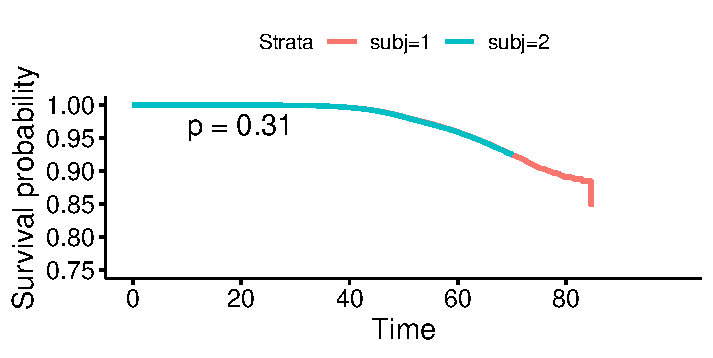
\includegraphics[width=0.7\linewidth]{PhD_thesis_template/plots/kmCompSis1.pdf}
    \includegraphics[width=0.7\linewidth]{PhD_thesis_template/plots/kmCompMom.pdf}
    \caption{Comparison among survival curves on main subject, first second and third sister, and mother.}
    \label{fig:my_label}
\end{figure}
\clearpage
\section*{Assumption validation}
\subsection*{Parameter estimation with no risk groups}
Before looking at the data we had few ideas on the nature of this topic, the breast cancer time and diagnosis. Very first of all we validate how likely could be to use the Weibull as the time-to-event distribution. We conduct parameter estimation through univariate and multivariate likelihood with Weibull distribution. In the end, we obtain the following results of the point estimates and their variances:
\begin{table}[ht]
\begin{tabular}{lcccc}
Model & $\widehat{shape}$ & var($\widehat{shape}$) & $\widehat{scale}$ & var($\widehat{scale}$) \\
univariate   &5.232 &1.2e-04 &110.901 &1e-03 \\
univariate on mothers &3.903 &4.433e-05 &148.594 &7.7e-04 \\
multivariate subj + mother &3.969 &2.599e-05 &143.928 &4.9e-04 \\
multivariate on all &4.018 &2.205e-05 &141.775 &4e-04
\end{tabular}
\caption{Parameter estimation from a Weibull time-to-event non-cure survival model}
\end{table}

The average time-to-event for the univariate and multivariate likelihood are respectively: 102.0919 and 127.9244. They show to be reliable for the Swedish Multi-Registries database taking into account that everybody will experience breast cancer eventually. In addition, the average time-to-event with the univariate likelihood is lower than the multivariate average time-to-event, as expected, because the in the multivariate model also mothers are considered and, due to their older age, they increase the average. 

But, we would like to validate the assumption of cure rate structure of the survival function. Results are promising for multiple reasons: the estimated cured fraction takes value different from zero (the degenerate case where everybody will experience the event) and the Weibull parameters have estimated values that are more likely to happen. Results in terms of estimated parameters and their variances are reported in the following lines: 
\begin{table}[ht]
\begin{tabular}{lcccccc}
Model &$\widehat{p}_0$ &var($\widehat{p}_0$) & \widehat{shape} & var(\widehat{shape}) & \widehat{scale} & var(\widehat{scale}) \\
univariate   &0.918 &1.584e-05 &6.6 &2.4e-04 &62.878 &6.8e-04 \\
univariate on mothers &0.869 &5.61e-06 &5.304 &8.017e-05 &77.558 &2.8e-04 \\
multivariate subj + mother &0.868 &4e-06 &5.285 &4.533e-05 &75.781 &1.8e-04 \\
multivariate on all &0.868 &3.51e-06 &5.345 &3.794e-05 &75.193 &1.5e-04
\end{tabular}
\caption{Parameter estimation from a Weibull time-to-event cure survival model}
\end{table}

Indeed, the average time-to-event decreases in this scenario in comparison to the non-cure-rate scenario. The mean time-to-event are, for the univariate and multivariate likelihood, respectively: 58.6358 and 69.28415.

These results are confirmed also by some interesting plots. We compare the Kaplan-Meier survival curve, which we can consider as the empirical description of our data, and the estimated survival curves, one with the classical structure and the other one with the cure rate structure. We build the plot for the main subjects, comparing the survival (cure rate and non-cure rate) fitted only on main subjects and on all subjects: 
\begin{figure}[ht]
    \centering
    \includegraphics[width=0.7\linewidth]{PhD_thesis_template/plots/mainKm.pdf}
    \caption{Kaplan-Meier for main subjects in comparison to estimated survival with and without cure rate, Weibull time-to-event, fitted on all family members.}
    \label{fig:my_label}
\end{figure}
\newline
\begin{figure}[ht]
    \centering
    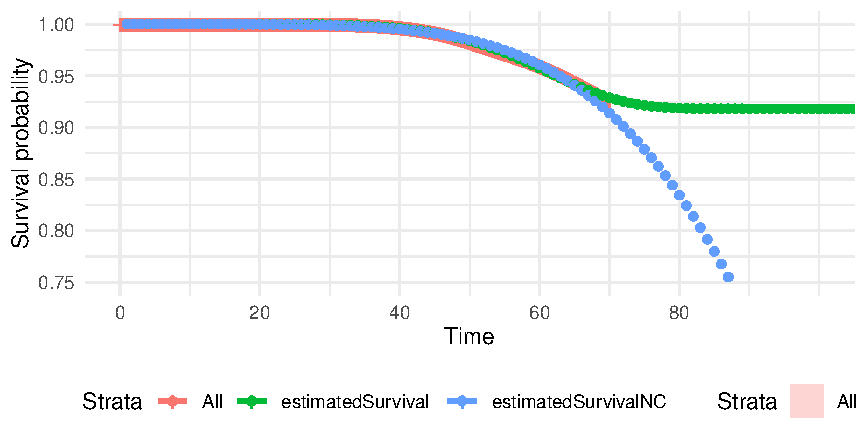
\includegraphics[width=0.7\linewidth]{PhD_thesis_template/plots/kmUnivariateMain.pdf}
    \caption{Kaplan-Meier for main subjects in comparison to estimated survival with and without cure rate, Weibull time-to-event, fitted on main subjects.}
    \label{fig:my_label}
\end{figure}
\newline
And the we repeat the same plot for only the mothers, where we can better appreciate the final plateau due to the likely cure rate structure of the dataset!
\begin{figure}[ht]
    \centering
    \includegraphics[width=0.7\linewidth]{PhD_thesis_template/plots/motherKm.pdf}
    \caption{Kaplan-Meier on mothers in comparison to estimated survival with and without cure rate, Weibull time-to-event, fitted on all family members.}
    \label{fig:my_label}
\end{figure}
\newline
Finally, the plot with main daughters and mothers is also reported to show a complete result, comparing the survival curves (cure rate and non-cure rate) fitted on both subjects and mothers and all subjects (i.e. sisters included): 
\begin{figure}[ht]
    \centering
    \includegraphics[width=0.7\linewidth]{PhD_thesis_template/plots/allKm.pdf}
    \caption{Kaplan-Meier on main subjects and mother in comparison to estimated survival with and without cure rate, Weibull time-to-event, fitted on all family members.}
    \label{fig:my_label}
\end{figure}
\newpage
\begin{figure}[ht]
    \centering
    \includegraphics[width=0.7\linewidth]{PhD_thesis_template/plots/kmMultiMainMother.pdf}
    \caption{Kaplan-Meier on main subjects and mother in comparison to estimated survival with and without cure rate, Weibull time-to-event, fitted on main subjects and mothers.}
    \label{fig:my_label}
\end{figure}
\newline
We also save the comparison with all subjects, with the survival curved fitted on all subjects: 
\begin{figure}[ht]
    \centering
    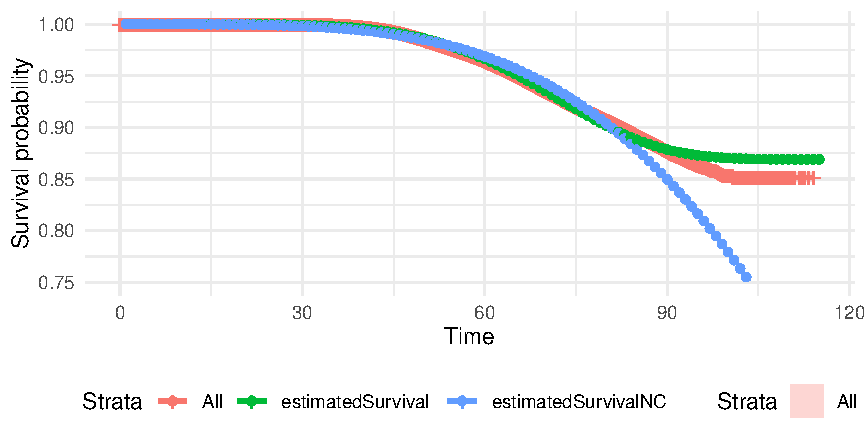
\includegraphics[width=0.7\linewidth]{PhD_thesis_template/plots/kmMultiAllSubjects.pdf}
    \caption{Kaplan-Meier on all subjects (sisters included) in comparison to estimated survival with and without cure rate, Weibull time-to-event, fitted on all subjects.}
    \label{fig:my_label}
\end{figure}
\newline

Now, we wonder whether the tail of the Kaplan-Meier is reliable. First of all, it should be reliable due to the precise data collection that is behind this dataset. But still, we double check through the Swedish life tables, available online \cite{swedishlifetable}. From the tables we focus on the ultracentenary ages of the years 2017 and 2018, that are the years right after the end of the follow-up time in our dataset. Hazard is on the fourth column while the survival is on the fifth. 
\begin{table}[ht]
\begin{tabular}{llllllllll}
Year & Age & & Hazard & Survival & & & & & \\
2017 & 100  & 0.44920 & 0.36682 & 0.50 & 2361 & 866 & 1928 & 4730 & 2.00 \\
2017 & 101  & 0.48769 & 0.39208 & 0.50 & 1495 & 586 & 1202 & 2801 & 1.87 \\
2017 & 102  & 0.52632 & 0.41667 & 0.50 & 909  & 379 & 720  & 1599 & 1.76 \\
2017 & 103  & 0.56464 & 0.44033 & 0.50 & 530  & 233 & 413  & 880  & 1.66 \\
2017 & 104  & 0.60220 & 0.46284 & 0.50 & 297  & 137 & 228  & 466  & 1.57 \\
2017 & 105  & 0.63860 & 0.48404 & 0.50 & 159  & 77  & 121  & 238  & 1.50 \\
2017 & 106  & 0.67347 & 0.50382 & 0.50 & 82   & 41  & 62   & 117  & 1.43 \\
2017 & 107  & 0.70652 & 0.52209 & 0.50 & 41   & 21  & 30   & 56   & 1.37 \\
2017 & 108  & 0.73754 & 0.53883 & 0.50 & 20   & 11  & 14   & 26   & 1.32 \\
2017 & 109  & 0.76635 & 0.55405 & 0.50 & 9    & 5   & 7    & 12   & 1.29 \\
2017 & 110+ & 0.79290 & 1.00000 & 1.26 & 4    & 4   & 5    & 5    & 1.26
\end{tabular}
\end{table}
\begin{table}[ht]
\begin{tabular}{llllllllll}
Year & Age & & Hazard & Survival & & & & & \\
2018 & 100  & 0.44675 & 0.36518 & 0.50 & 2487 & 908 & 2033 & 5000 & 2.01 \\
2018 & 101  & 0.48551 & 0.39067 & 0.50 & 1579 & 617 & 1270 & 2967 & 1.88 \\
2018 & 102  & 0.52444 & 0.41549 & 0.50 & 962  & 400 & 762  & 1697 & 1.76 \\
2018 & 103  & 0.56309 & 0.43938 & 0.50 & 562  & 247 & 439  & 935  & 1.66 \\
2018 & 104  & 0.60098 & 0.46212 & 0.50 & 315  & 146 & 242  & 496  & 1.57 \\
2018 & 105  & 0.63770 & 0.48353 & 0.50 & 170  & 82  & 129  & 254  & 1.50 \\
2018 & 106  & 0.67288 & 0.50349 & 0.50 & 88   & 44  & 66   & 125  & 1.43 \\
2018 & 107  & 0.70621 & 0.52192 & 0.50 & 43   & 23  & 32   & 60   & 1.37 \\
2018 & 108  & 0.73748 & 0.53880 & 0.50 & 21   & 11  & 15   & 28   & 1.32 \\
2018 & 109  & 0.76652 & 0.55414 & 0.50 & 10   & 5   & 7    & 12   & 1.29 \\
2018 & 110+ & 0.79324 & 1.00000 & 1.26 & 4    & 4   & 5    & 5    & 1.26
\end{tabular}
\end{table}

The life table result must be replicated by our dataset. If the tail is reliable, this means that ultracentenary subjects are truly still alive by the end of the study and they have their censoring event (either death or emigration) just after the end of the follow-up. If the recorded data are correct we expect to find a similar proportion of how many died in those years. Trivially, we only consider censoring until the 2018 because we do not have any information further. 

To better explain, if these subjects have their death date recorded in the dataset between the end of the follow-up (last day of 2016) and the 2018, we are guaranteed that they were alive for all the follow-up time (i.e. in the tail), being truly a censored event. If this is not the case, there could be a problem of missing data. The hazard of dying after being centenary is in mean 0.5315. We compute the proportion of deaths in the biennal out of the total of alive people. The result is 0.5037, that is very similar to the life table one. From these results we can claim that the cure rate assumption holds, because of the presence of old alive women that do not experience the event breast cancer eventually, no matter how long they will live). For completeness of results, We report the table of the ultracentenary women below.
\begin{table}[ht]
\begin{tabular}{llllllll}
100   & 101   & 102   & 103   & 104   & 105   & 106   & 107 \\
\hline
0.226 & 0.326 & 0.150 & 0.103 & 0.053 & 0.033 & 0.040 & 0.018 \\\\
108   & 109   & 110   & 111   & 112   & 113   & 114   \\
\hline
0.013 & 0.013 & 0.008 & 0.005 & 0.008 & 0.005 & 0.003
\end{tabular}
\end{table}

Model with FH with no latent variable, the results from the univariate likelihood are: 
model alpha p0 shape scale 
univariate 0.69096864 0.0027219 0.92075716 3.8e-05 6.59416891 1.842e-05 62.88303038 1.48e-06
multivariate 

Once that we estimated parameters from the model with the known family history indicator we can distinguish two risk groups that follow the cure rate structure. One can compare the probability of belonging to the low risk group to the probability of belonging to the high risk group. We may assess whether each observation is more likely to belong to a Weibull cure rate model with the low risk parameters or to the same distribution but with the high risk parameters ($\alpha$ is added to th model). Can we compare the densities on the same times and then compare these two densities for each observation?  

\subsection*{Alternative distributions}
We repeat the analysis above with the Gamma and the logNormal distribution instead of the Weibull. In the end of the analysis we compare the goodness of fit among these distributions through the Akaike information criterios (aic). 

First, we proceed with the Gamma distribution. Results from the parameter estimation with the non-cure model are reported in the following table: 
\begin{table}[ht]
\begin{tabular}{lcccc}
Model & \widehat{shape} & var(\widehat{shape}) & \widehat{scale} & var(\widehat{scale}) \\
univariate on subjects  &8.323 &0.00042289 &14.884 &0.00162094 \\
univariate on mothers &5.995 &0.00014461 &26.439 &0.0013604 \\
multivariate subj + mother &6.103 &8.628e-05 &25.155 &0.00079255 \\
multivariate &6.207 &7.439e-05 &24.375 &0.00065382
\end{tabular}
\caption{Parameter estimation from a Gamma time-to-event non-cure survival model.}
\end{table}
\newpage

Similarly, results from the cure-rate scenario are reported in the table. Notice that now there is the additional parameter which indicates the cured fraction. \begin{table}[ht]
\begin{tabular}{lcccccc}
Model &$\widehat{p}_0$ & var($\widehat{p}_0$) & \widehat{shape} & var(\widehat{shape}) & \widehat{scale} & var(\widehat{scale}) \\
univariate on subjects  &0.871 &9.796e-05 &15.794 &0.00427274 &4.353 &0.00242267 \\
univariate on mothers &0.838 &1.684e-05 &13.257 &0.00116014 &5.97 &0.00092954 \\
multivariate subj + mother &0.841 &1.103e-05 &13.092 &0.00065214 &5.87 &0.00053817 \\
multivariate &0.842 &9.73e-06 &13.204 &0.0005536 &5.776 &0.00044842
\end{tabular}
\caption{Parameter estimation from a Gamma time-to-event cure survival model.}
\end{table}
A graphical representation of the comparison among the Kaplan-Meier on the data and the estimated survival cure and non-cure is reported in the following pictures. 
\begin{figure}[ht]
    \centering
    \includegraphics[width=0.7\linewidth]{PhD_thesis_template/plots/kmUniSubGamma.pdf}
    \caption{Kaplan-Meier on main subjects in comparison to estimated survival with and without cure rate, fitted on main subjects}
    \label{fig:my_label}
\end{figure}
\newline
\begin{figure}[ht]
    \centering
    \includegraphics[width=0.7\linewidth]{PhD_thesis_template/plots/kmUniMotherGamma.pdf}
    \caption{Kaplan-Meier on mothers in comparison to estimated survival with and without cure rate, fitted on mothers}
    \label{fig:my_label}
\end{figure}
\newline
\begin{figure}[ht]
    \centering
    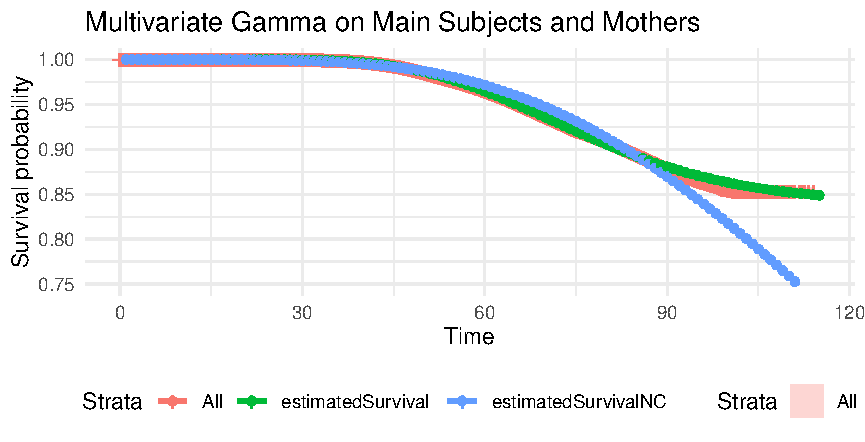
\includegraphics[width=0.7\linewidth]{PhD_thesis_template/plots/kmMultiSubMotherGamma.pdf}
    \caption{Kaplan-Meier on subjects and mothers in comparison to estimated survival with and without cure rate, fitted on subjetcs and mothers}
    \label{fig:my_label}
\end{figure}
\newline
\begin{figure}[ht]
    \centering
    \includegraphics[width=0.7\linewidth]{PhD_thesis_template/plots/kmMultiAllGamma.pdf}
    \caption{Kaplan-Meier on all in comparison to estimated survival with and without cure rate, fitted on subjetcs and mothers}
    \label{fig:my_label}
\end{figure}
\newpage
Lastly, we collect results from the LogNormal distribution on the time-to-event. Results from the parameter estimation with the non-cure model are reported in the following table: 
\begin{table}[ht]
\begin{tabular}{lcccc}
Model & $\widehat{\mu}$ & var($\widehat{\mu}$) & $\widehat{\sigma}$ & var($\widehat{\sigma}$) \\
univariate on subjects  &4.883 &1.605e-05 &0.454 &9.29e-06 \\
univariate on mothers &5.109 &7.32e-06 &0.536 &5.17e-06 \\
multivariate subj + mother &5.082 &5.04e-06 &0.534 &3.11e-06 \\
multivariate &5.067 &4.32e-06 &0.529 &2.61e-06
\end{tabular}
\caption{Parameter estimation from a LogNormal time-to-event non-cure survival model.}
\end{table}
\newpage
Similarly, results from the cure-rate scenario are reported in the table. Notice that now there is the additional parameter which indicates the cured fraction. \begin{table}[ht]
\begin{tabular}{lcccccc}
Model &$\widehat{p}_0$ & var($\widehat{p}_0$) & $\widehat{\mu}$ & var($\widehat{\mu}$) & $\widehat{\sigma}$ & var($\widehat{\sigma}$) \\
univariate on subjects &0.825 &2.9e-04 &4.313 &1.3e-04 &0.31 &4.57e-05 \\
univariate on mothers &0.809 &3.756e-05 &4.41 &2.385e-05 &0.324 &1.341e-05 \\
multivariate subj + mother &0.812 &2.444e-05 &4.383 &1.557e-05 &0.328 &7.93e-06 \\
multivariate &0.857 &1.65e-06 &5.91 &3.688e-05 &1.847 &9.11e-06
\end{tabular}
\caption{Parameter estimation from a LogNormal time-to-event cure survival model.}
\end{table}
Results from the last scenario must be checked. Plus, a graphical representation of the comparison among the curves is reported in the following plots. 
\begin{figure}[ht]
    \centering
    \includegraphics[width=0.7\linewidth]{PhD_thesis_template/plots/kmUniSubLognormal.pdf}
    \caption{Kaplan-Meier on main subjects in comparison to estimated survival with and without cure rate, fitted on main subjects}
    \label{fig:my_label}
\end{figure}
\newline
\begin{figure}[ht]
    \centering
    \includegraphics[width=0.7\linewidth]{PhD_thesis_template/plots/kmUniMotherLognormal.pdf}
    \caption{Kaplan-Meier on mothers in comparison to estimated survival with and without cure rate, fitted on mothers}
    \label{fig:my_label}
\end{figure}
\newline
\begin{figure}[ht]
    \centering
    \includegraphics[width=0.7\linewidth]{PhD_thesis_template/plots/kmMultiSubMotherLognormal.pdf}
    \caption{Kaplan-Meier on subjects and mothers in comparison to estimated survival with and without cure rate, fitted on subjetcs and mothers}
    \label{fig:my_label}
\end{figure}
\newline
\begin{figure}[ht]
    \centering
    \includegraphics[width=0.7\linewidth]{PhD_thesis_template/plots/kmMultiAllLognormal.pdf}
    \caption{Kaplan-Meier on all in comparison to estimated survival with and without cure rate, fitted on all subjects (sisters included).}
    \label{fig:my_label}
\end{figure}
\newline
Since not promising results come out from the case where we include all the sisters, we additionally fit the cure and non-cure survival model only on the first sister to observe their behaviour. Results from different cases are reported below: 
\begin{table}[ht]
    \centering
    \begin{tabular}{lccccccc}
    Model &$\widehat{p}_0$ & var($\widehat{p}_0$) & $\widehat{\mu}$ & var($\widehat{\mu}$) & $\widehat{\sigma}$ & var($\widehat{\sigma}$) &AIC \\
    univariate on first sister (non-cure) & & &4.903 &3.908e-05 &0.461 &2.305e-05 &169459.7 \\
    univariate on first sister (cure) &0.79 &8e-04 &4.37 &3e-04 &0.325 &1e-04 &169217.9
    \end{tabular}
    \caption{Parameter estimation from a LogNormal time-to-event cure survival model on the first sister.}
    \label{tab:my_label}
\end{table}
A graphical representation is also reported: \begin{figure}
    \centering
    \includegraphics[width=0.7\linewidth]{PhD_thesis_template/plots/kmUniFirstSisterLognormal.pdf}
    \caption{Kaplan-Meier only on the first sister in comparison to estimated survival with and without cure rate, fitted on the first sister only.}
    \label{fig:my_label}
\end{figure}
\clearpage
Due to the bad performance of the two-parameters LogNormal, we move to the three-parameters LogNormal in order to gain the flexibility that we may need in this situation to fit better the model to the data. The additional parameter of the LogNormal is the threshold that indicates the starting time. Before the starting time the density function takes value zero and this might help in reducing the heavy right tail of the LogNormal distribution. We observe the results from the table below, where we can appreciate an improvement in the estimation procedure. \begin{table}[ht]
    \centering
    \begin{tabular}{lcccccccc}
         Model &$\widehat{p}_0$ & var($\widehat{p}_0$) & $\widehat{\mu}$ & var($\widehat{\mu}$) & $\widehat{\sigma}$ & var($\widehat{\sigma}$) &$\widehat{\gamma}$ &var($\widehat{\gamma}$)  \\
         multi 4 (non-cure) & & &0.774 &5.07e-06 &5.135 &1.99e-06 &18.342 &4e-03  \\
         multi (non-cure) & & &0.774 &5.07e-06 &5.134 &1.98e-06 &18.34 &4e-03 \\
         multi 4 (cure) &0.798 &5.7e-05 &0.373 &3.49e-05 &4.340 &6.05e-06 &5.441 &0.308  \\ 
         multi (cure) &0.798 &6.496e-05 &0.372 &1e-04 &4.345 &6.85e-06 &5.161 &0.430
    \end{tabular}
    \caption{Parameter estimation from a three-parameters LogNormal time-to-event usual and cure rate survival model.}
    \label{tab:my_label}
\end{table}
The representation of the comparison between the estimated survival is in the figure below. \begin{figure}
    \centering
    \includegraphics[width=0.7\linewidth]{PhD_thesis_template/plots/kmMulti4mem3Lognormal.pdf}
    \caption{Kaplan-Meier on the subject, mother and first two sisters in comparison to estimated 3-pars LogNormal survival with and without cure rate, fitted on subject, mother and first two sisters.}
    \label{fig:my_label}
\end{figure}
\clearpage
\begin{figure}[ht]
    \centering
    \includegraphics[width=0.7\linewidth]{PhD_thesis_template/plots/kmMultiAll3Lognormal.pdf}
    \caption{Kaplan-Meier on all subjects in comparison to estimated 3-pars LogNormal survival with and without cure rate, fitted on all subjects.}
    \label{fig:my_label}
\end{figure}
Also, three-parameters Gamma distribution is analysed to make a comparison with the LogNormal three-parameters. Shape anche scale of the Gamma are called $\mu$ and $\sigma$ respectively, and $\gamma$ is the shift. \begin{table}[ht]
    \centering
    \begin{tabular}{lccccccccc}
         Model &$\widehat{p}_0$ & var($\widehat{p}_0$) & $\widehat{\mu}$ & var($\widehat{\mu}$) & $\widehat{\sigma}$ & var($\widehat{\sigma}$) &$\widehat{\gamma}$ &var($\widehat{\gamma}$) \\
         multi 4 (non-cure) & & &3.277 &1e-04 &47.051 &1e-03 &21.065 &1.6e-04  \\
         multi (non-cure) & & &3.285 &1e-04 &46.822 &1.5e-03 &21.066 &1.3e-04  \\
         multi 4 (cure) &0.827 &1.75e-05 &8.326 &1.4e-02 &8.229 &1.7e-03 &11.189 &7e-02  \\
         multi (cure) &0.828 &1.69e-05 &8.345 &1e-02 &8.199 &1.6e-03 &11.197 &6.7e-02  \\
    \end{tabular}
    \caption{Parameter estimation from a three-parameters Gamma time-to-event cure survival model.}
    \label{tab:my_label}
\end{table}
The results are represented in the picture below: \begin{figure}[ht]
    \centering
    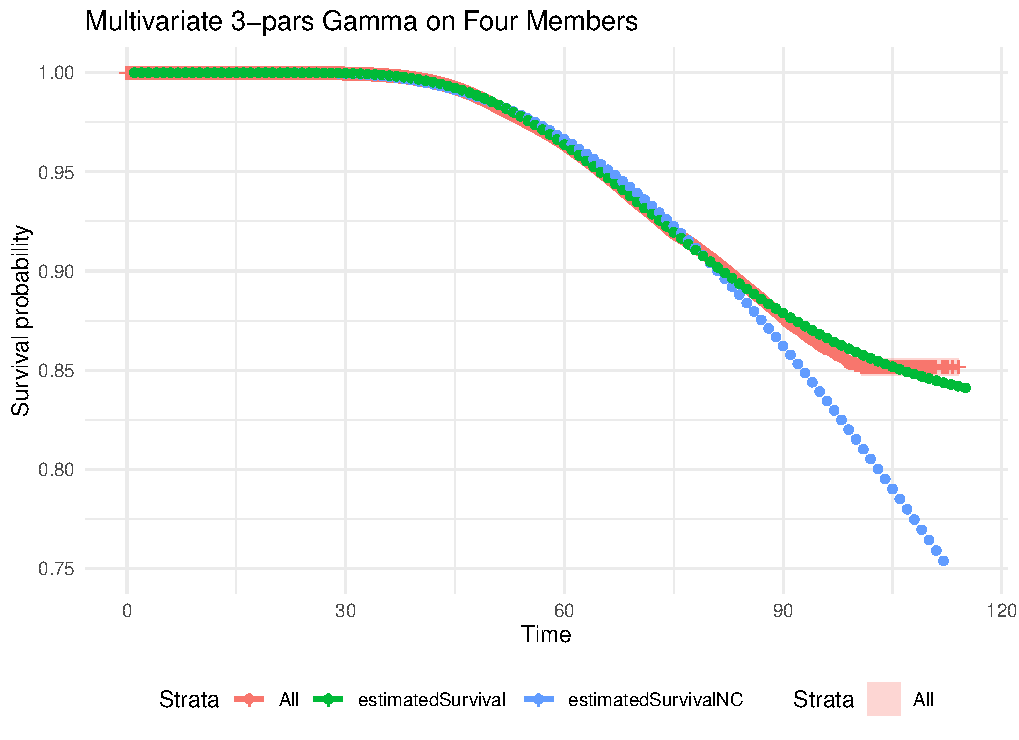
\includegraphics[width=0.7\linewidth]{PhD_thesis_template/plots/kmMulti4mem3Gamma.pdf}
    \caption{Kaplan-Meier on the subject, mother and first two sisters in comparison to estimated 3-pars Gamma survival with and without cure rate, fitted on subject, mother and first two sisters.}
    \label{fig:my_label}
\end{figure}
\clearpage
\begin{figure}[ht]
    \centering
    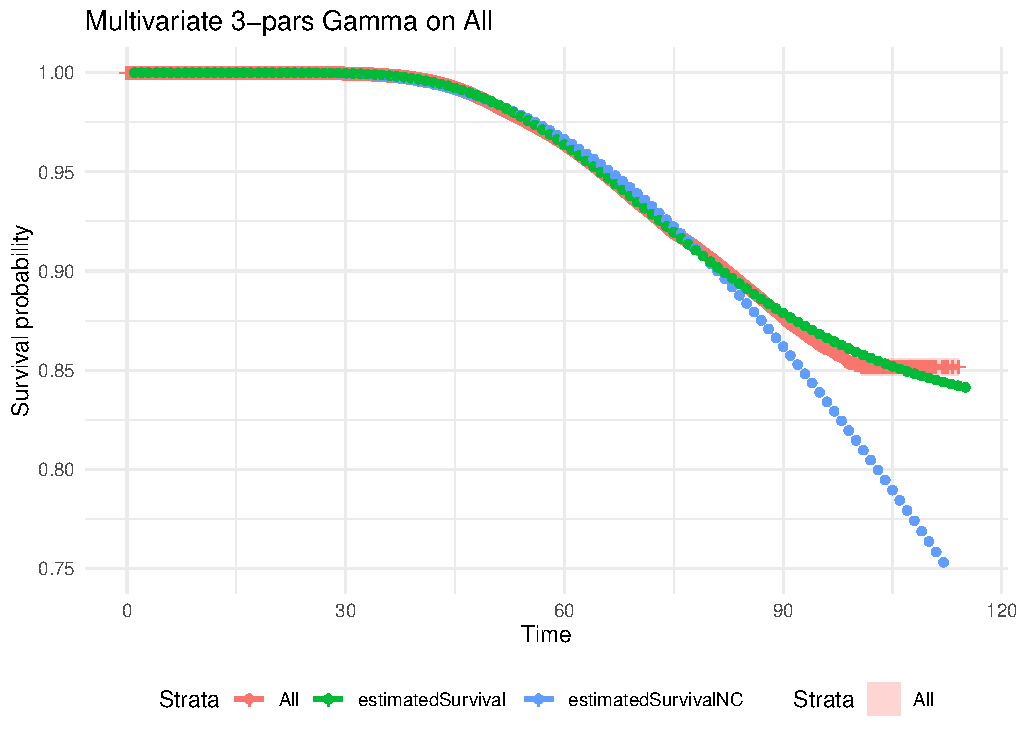
\includegraphics[width=0.7\linewidth]{PhD_thesis_template/plots/kmMultiAll3Gamma.pdf}
    \caption{Kaplan-Meier on all subjects in comparison to estimated 3-pars Gamma survival with and without cure rate, fitted on all subjects.}
    \label{fig:my_label}
\end{figure}
The complete analysis brings us to conclude that the three-parameters Gamma distribution is not needed, because the model with two parameters already perform a good fitting and the third parameter affects the results in a negative way, in terms of accuracy in estimating the Kaplan-Meier, indeed $p_0$ from the two-parameters is closer to the K-M cured fraction () than the one from the three-parameters: 0.842 (9.73e-06) versus 0.828 (1.696e-05) respectively. In terms of AIC they have very similar values as: 1688066 (two-parameters) versus 1687749 (three-parmeters). The difference is not significant to make us choose adding the shifting parameter into the model. 

A comparison among the distributions is made through the AIC. The model with the lowest AIC is selected as the best fitting. Results about the selection indicator AIC are collected in the following table: 
\begin{table}[ht]
\begin{tabular}{llcc}
Distribution &Model &AIC &  \\ \hline
Weibull & &non-cure &cure \\
\hline
&univariate on subjects &440685.6 &439053.4  \\
&univariate on mothers &1032613 &1026155 \\
&multivariate subj + mother &1478542  &1467965 \\
&multivariate &1705353 &1692822 \\ \hline
Gamma & &non-cure &cure \\
\hline
&univariate on subjects &439516 &438391.8  \\
&univariate on mothers &1029223 &1023994 \\
&multivariate subj + mother &1472628 &1463964 \\
&multivariate &1698245 &\colorbox{yellow}{1688066} \\ \hline
LogNormal & &non-cure &cure \\
\hline
&univariate on subjects &\textbf{438958.8} &\textbf{438368.4}\\
&univariate on mothers &\textbf{1027040} &\textbf{1023771} \\
&multivariate subj + mother &\textbf{1468891} &\textbf{1463539} \\
&multivariate &\textbf{1693854} &2334626 \\ \hline
Gamma 3-pars & &non-cure &cure \\
\hline
&multivariate on 4 subjects &1694186 &1674377 \\ 
&multivariate &1707589 &1687749 \\ \hline
LogNormal 3-pars & &non-cure &cure \\
\hline
&multivariate on 4 subjects &1684866 &\textbf{1674185} \\
&multivariate &1698257 &\colorbox{yellow}{\textbf{1687555}}
\end{tabular}
\caption{AIC comparison among different distributions.}
\end{table}
\newline
According to the likelihood used the best-fit model varies. Following the order from top to bottom in the column ``Model'' into the above table, the best-fit model is the LogNormal. The LogNormal model seems to be the best-fit model for all the scenarios but not when maximizing the Multivariate Likelihood on all subjects with cure rate survival function, scenario where the Gamma distribution shows the lowest AIC.

We can conclude that the best-fit model with two parameters is the Gamma. The third parameter in the Gamma distribution is not bringing to a significant change in the fitting if we comapare the results in terms of AIC. While instead, the third parameter has been involved in the modelling process to solve the bad-fit of the two-parameters LogNormal, and it seems to work in the preferred direction. Most importantly, this analysis allows us to use the cure rate model as the proper one for this kind of data. But, up to here we can not say anything about the family latent risk of having breast cancer. Due to this reason, we move to the analysis with two latent risk groups. 

\subsection*{Parameter estimation with risk groups}
We assume that two risk groups exist in the Swedish Multi-Registries dataset. We perform parameter estimation to assess whether the past hypothesis can be reliable or not. It is possible that two risk groups in this dataset are too much reductive since we already now that the risk of having breast cancer has been modelled as continuous. 

Parameter estimation is performed as above on four different scenarios: univariate only on main subjects, univariate only on mothers, multivariate on main subjects and mothers, and multivariate on all subjects (sisters included). For each scenario both the survival function cure rate and non-cure rate are estimated, and later compared with the Kaplan-Meier on real data (the same used for the estimation procedure). The three different distributions of above: Weibull, Gamma, and LogNormal are compared through the AIC in the end of analysis.

We collect results from the Weibull distribution on the time-to-event. Results from the parameter estimation with the non-cure model are reported in the following table. For a matter of space we call the shape and scale of the Weibull with the symbols: $\mu$, and $\sigma$.
\begin{table}[ht]
\begin{tabular}{lcccccccc}
Model & $\widehat{\mu}$ & var($\widehat{\mu}$) & $\widehat{\sigma}$ & var($\widehat{\sigma}$) &$\widehat{\alpha}$ &var($\widehat{\alpha}$) &$\widehat{h}$ &var($\widehat{h}$)  \\
univariate on subjects  &&&&&&&& \\
univariate on mothers &&&&&&&& \\
multivariate subj + mother &&&&&&&& \\
multivariate &&&&&&&&
\end{tabular}
\caption{Parameter estimation from a baseline Weibull non-cure survival function.}
\end{table}
\newline
Similarly, results from the cure-rate scenario are reported in the table. Notice that now there is the additional parameter which indicates the cured fraction. For a matter of space we call the shape and scale of the Weibull with the symbols: $\mu$, and $\sigma$. \begin{table}[ht]
\begin{tabular}{lcccccccccc}
Model &$\widehat{p}_0$ & var($\widehat{p}_0$) &  $\widehat{\mu}$ & var($\widehat{\mu}$) &$\widehat{\sigma}$ & var($\widehat{\sigma}$) &$\widehat{\alpha}$ &var($\widehat{\alpha}$) &$\widehat{h}$ &var($\widehat{h}$)  \\
univariate on subjects &&&&&&&& \\
univariate on mothers &&&&&&&& \\
multivariate subj + mother &&&&&&&& \\
multivariate &&&&&&&&
\end{tabular}
\caption{Parameter estimation from a baseline Weibull cure survival function.}
\end{table}
The same analysis is repeated for the Gamma distribution, where shape and scale of the Gamma are represented with $\mu$ and $\sigma$ respectively. 
\begin{table}[ht]
\begin{tabular}{lcccccccc}
Model & $\widehat{\mu}$ & var($\widehat{\mu}$) & $\widehat{\sigma}$ & var($\widehat{\sigma}$) &$\widehat{\alpha}$ &var($\widehat{\alpha}$) &$\widehat{h}$ &var($\widehat{h}$)  \\
univariate on subjects  &&&&&&&& \\
univariate on mothers &&&&&&&& \\
multivariate subj + mother &&&&&&&& \\
multivariate &&&&&&&&
\end{tabular}
\caption{Parameter estimation from a baseline Gamma non-cure survival function.}
\end{table}
\newline
Similarly, results from the cure-rate scenario are reported in the table. Notice that now there is the additional parameter which indicates the cured fraction. For a matter of space we call the shape and scale of the Weibull with the symbols: $\mu$, and $\sigma$. \begin{table}[ht]
\begin{tabular}{lcccccccccc}
Model &$\widehat{p}_0$ & var($\widehat{p}_0$) &  $\widehat{\mu}$ & var($\widehat{\mu}$) &$\widehat{\sigma}$ & var($\widehat{\sigma}$) &\widehat{\alpha} &var(\widehat{\alpha}) &\widehat{h} &var(\widehat{h})  \\
univariate on subjects &&&&&&&& \\
univariate on mothers &&&&&&&& \\
multivariate subj + mother &&&&&&&& \\
multivariate &&&&&&&&
\end{tabular}
\caption{Parameter estimation from a baseline Gamma cure survival function.}
\end{table}
Lastly, the analysis is repeated for the LogNormal distribution that gives the following results: 
\begin{table}[ht]
\begin{tabular}{lcccccccc}
Model & $\widehat{\mu}$ & var($\widehat{\mu}$) & $\widehat{\sigma}$ & var($\widehat{\sigma}$) &\widehat{\alpha} &var(\widehat{\alpha}) &\widehat{h} &var(\widehat{h})  \\
univariate on subjects  &&&&&&&& \\
univariate on mothers &&&&&&&& \\
multivariate subj + mother &&&&&&&& \\
multivariate &&&&&&&&
\end{tabular}
\caption{Parameter estimation from a baseline LogNormal non-cure survival function.}
\end{table}
\newline
Similarly, results from the cure-rate scenario are reported in the table. Notice that now there is the additional parameter which indicates the cured fraction. For a matter of space we call the shape and scale of the Weibull with the symbols: $\mu$, and $\sigma$. \begin{table}[ht]
\begin{tabular}{lcccccccccc}
Model &$\widehat{p}_0$ & var($\widehat{p}_0$) &  $\widehat{\mu}$ & var($\widehat{\mu}$) &$\widehat{\sigma}$ & var($\widehat{\sigma}$) &\widehat{\alpha} &var(\widehat{\alpha}) &\widehat{h} &var(\widehat{h})  \\
univariate on subjects &&&&&&&& \\
univariate on mothers &&&&&&&& \\
multivariate subj + mother &&&&&&&& \\
multivariate &&&&&&&&
\end{tabular}
\caption{Parameter estimation from a baseline LogNormal cure survival function.}
\end{table}

From the AIC results below, we can notice that the best-fit model is the LogNormal. 
\begin{table}[ht]
\begin{tabular}{llcc}
Distribution &Model &AIC &  \\ \hline
Weibull & &non-cure &cure \\
\hline
&univariate on subjects &&  \\
&univariate on mothers && \\
&multivariate subj + mother && \\
&multivariate && \\ \hline
Gamma & &non-cure &cure \\
\hline
&univariate on subjects &&  \\
&univariate on mothers && \\
&multivariate subj + mother && \\
&multivariate && \\ \hline
LogNormal & &non-cure &cure \\
\hline
&univariate on subjects && \\
&univariate on mothers && \\
&multivariate subj + mother && \\
&multivariate &&
\end{tabular}
\caption{AIC comparison among different distributions.}
\end{table}
\newpage

\section*{Notes}
We explore different scenarios in terms of cure rate model or usual survival model, and number of risk groups like no groups, two groups and continuous frailty. We show the scenarios we want to explore below: \begin{table}[ht]
\begin{tabular}{llll}
                             & No risk groups        & R = 0/1               & Continuous Frailty         \\ \cline{2-4} 
\multicolumn{1}{l|}{Cure}    & \multicolumn{1}{l|}{done before} & \multicolumn{1}{l|}{} & \multicolumn{1}{l|}{} \\ \cline{2-4} 
\multicolumn{1}{l|}{No Cure} & \multicolumn{1}{l|}{done before} & \multicolumn{1}{l|}{} & \multicolumn{1}{l|}{} \\ \cline{2-4} 
\end{tabular}
\end{table}
\newline 
We collect some results in the following lines. We notice that plain parameter estimation is not robust, then a penalization can help in estimating the parameters. We want to assess whether we can find two risk groups or, at the contrary, this is an unlikely hypothesis for this dataset. 

We set five random values for each of the parameters: \begin{table}[ht]
\centering
\begin{tabular}{rrrrrr}
  \hline
 & pVals & shVals & scVals & aVals & hVals \\ 
  \hline
1 & 0.638 & 9.926 & 49.444 & 0.941 & 0.361 \\ 
  2 & 0.581 & 9.001 & 49.408 & 0.161 & 0.898 \\ 
  3 & 0.788 & 11.993 & 50.904 & 0.546 & 0.392 \\ 
  4 & 0.927 & 10.472 & 49.195 & 0.335 & 0.178 \\ 
  5 & 0.003 & 10.551 & 51.621 & 0.895 & 0.488 \\ 
   \hline
\end{tabular}
\end{table}
\newline
And we save in the tables below the value of the likelihood (column 1), the punctual estimate (columns 2-6) and the variance for each of the parameter (columns 7-11). The penalization is absent or it is varying with the form $\lambda\cdot 1/\alpha$ with lambda assuming the values $\lambda = 1,2,5,20$. From these simulations we can moreover have an additional proof of the identifiability of the model, if the estimates are stable from different starting point in the estimation algorithm, and different strength of penalization. 
\begin{table}[ht]
\centering
\begin{tabular}{rrrrrrrrrrr}
  \hline
 1 & 2 & 3 & 4 & 5 & 6 & 7 & 8 & 9 & 10 & 11 \\ 
  \hline
 834532.255 & 0.918 & 4.881 & 78.959 & 0.082 & 0.113 & 0.000 & 0.000 & 0.000 & 0.000 & 0.000 \\ 
 816884.902 & 1.000 & 5.025 & 73.144 & 0.000 & 0.705 & 0.000 & 0.000 & 0.000 & 0.000 & 0.000 \\ 
 817075.072 & 1.000 & 5.006 & 73.057 & 0.002 & 0.814 & 0.000 & 0.000 & 0.000 & 0.000 & 0.000 \\ 
 816884.738 & 1.000 & 5.025 & 73.125 & 0.000 & 0.706 & 0.000 & 0.000 & 0.000 & 0.000 & 0.000 \\ 
 818152.699 & 0.997 & 4.959 & 71.855 & 0.020 & 1.000 & 0.000 & 0.000 & 0.000 & 0.000 & -440.509 \\
   \hline
\end{tabular}
\caption{$\lambda = 0$}
\end{table}
\begin{table}[ht]
\centering
\begin{tabular}{rrrrrrrrrrr}
  \hline
 1 & 2 & 3 & 4 & 5 & 6 & 7 & 8 & 9 & 10 & 11 \\ 
  \hline
 846364.239 & 0.869 & 5.339 & 75.187 & 0.998 & 0.756 & 0.000 & 0.000 & 0.000 & -0.023 & 0.179 \\ 
  817534.343 & 0.999 & 4.999 & 73.022 & 0.006 & 0.909 & 0.000 & 0.000 & 0.000 & 0.000 & 0.001 \\ 
 825961.017 & 0.062 & 3.495 & 627.295 & 0.006 & 0.998 & 0.002 & 0.000 & 0.000 & 0.000 & -0.171 \\ 
  817714.300 & 0.999 & 5.003 & 72.855 & 0.005 & 1.000 & 0.000 & 0.000 & 0.000 & 0.000 & -2.681 \\ 
  817574.622 & 0.999 & 5.040 & 73.172 & 0.003 & 0.585 & 0.000 & 0.000 & 0.000 & 0.000 & 0.000 \\
   \hline
\end{tabular}
\caption{$\lambda = 1$}
\end{table}
\begin{table}[ht]
\centering
\begin{tabular}{rrrrrrrrrrr}
  \hline
1 & 2 & 3 & 4 & 5 & 6 & 7 & 8 & 9 & 10 & 11 \\ 
  \hline
846365.241 & 0.869 & 5.339 & 75.187 & 0.998 & 0.756 & 0.000 & 0.000 & 0.000 & -0.023 & 0.179 \\ 
 817620.280 & 0.999 & 5.018 & 73.004 & 0.007 & 0.861 & 0.000 & 0.000 & 0.000 & 0.000 & 0.000 \\ 
  826110.270 & 0.066 & 3.498 & 563.303 & 0.008 & 0.997 & 0.002 & 0.000 & 0.000 & 0.000 & -0.156 \\ 
 817869.327 & 0.999 & 5.001 & 72.897 & 0.008 & 1.000 & 0.000 & 0.000 & 0.000 & 0.000 & -1.761 \\ 
 817538.378 & 0.998 & 5.000 & 73.092 & 0.007 & 0.683 & 0.000 & 0.000 & 0.000 & 0.000 & 0.000 \\ 
   \hline
\end{tabular}
\caption{$\lambda = 2$}
\end{table}
\begin{table}[ht]
\centering
\begin{tabular}{rrrrrrrrrrrr}
  \hline
1 & 2 & 3 & 4 & 5 & 6 & 7 & 8 & 9 & 10 & 11 \\ 
  \hline
846368.248 & 0.869 & 5.339 & 75.187 & 0.998 & 0.756 & 0.000 & 0.000 & 0.000 & -0.023 & 0.179 \\ 
817915.982 & 0.998 & 5.028 & 73.026 & 0.011 & 0.827 & 0.000 & 0.000 & 0.000 & 0.000 & 0.000 \\ 
826402.378 & 0.088 & 3.496 & 495.065 & 0.013 & 0.996 & 0.001 & 0.000 & 0.000 & 0.000 & -0.121 \\ 
818176.835 & 0.998 & 5.001 & 72.897 & 0.012 & 1.000 & 0.000 & 0.000 & 0.000 & 0.000 & -1.111 \\ 
818010.407 & 0.998 & 4.996 & 73.102 & 0.009 & 0.627 & 0.000 & 0.000 & 0.000 & 0.000 & 0.000 \\ 
   \hline
\end{tabular}
\caption{$\lambda = 5$}
\end{table}
\begin{table}[ht]
\centering
\begin{tabular}{rrrrrrrrrrr}
  \hline
1 & 2 & 3 & 4 & 5 & 6 & 7 & 8 & 9 & 10 & 11 \\ 
  \hline
846383.285 & 0.869 & 5.339 & 75.187 & 0.998 & 0.756 & 0.000 & 0.000 & 0.000 & -0.023 & 0.179 \\ 
818867.961 & 0.995 & 5.064 & 73.118 & 0.021 & 0.713 & 0.000 & 0.000 & 0.000 & 0.000 & 0.000 \\ 
826647.708 & 0.806 & 3.600 & 233.012 & 0.022 & 0.661 & 0.000 & 0.000 & 0.000 & 0.000 & 0.000 \\ 
819012.106 & 0.996 & 5.010 & 72.943 & 0.024 & 0.999 & 0.000 & 0.000 & 0.000 & 0.000 & -0.674 \\ 
818829.831 & 0.996 & 5.020 & 73.169 & 0.021 & 0.786 & 0.000 & 0.000 & 0.000 & 0.000 & 0.000 \\ 
   \hline
\end{tabular}
\caption{$\lambda = 20$}
\end{table}
\newpage
Results from above can express the absence of two risk groups, as we could expect from the beginning since the risk is likely to be continuous frailty or the presence of a multi-modal likelihood that indeed could be maximized in different points of the grid of values. Instead of varying all the parameters starting point for the likelihood exploration, we fix four values out of five and we explore one parameter estimation at the time. We start with $p_0$, saving the value of the likelihood and the value of $\widehat{p}_0$.

Results are saved in the following table where there are the fixed values and the solo estimated parameters one at the time. We then find on the diagonal the estimated parameters. 

We thought that we need more flexibility in these data, for its complexity and also because they bring a lot of information due to its dimension. Probably there are not two risk groups following the previous trials, and k-groups neither. That is why we move to a continuous frailty. In addition, the advantage of this approach is its availability in the main statistical softwares where also the posterior (empirical Bayes) estimates of the frailty for each cluster can be computed. The cluster is the family, since we assume that the risk of having breast cancer is familiar.  
\bibliography{biblio}
\end{document}